\documentclass{../qh_assignment}
\graphicspath{ {./images/} }

\begin{document}

\section{Koch's Curve generatie 1}
Maak de functie
\begin{lstlisting}
	void kochCurve(PVector p1, PVector p2) {
	}
\end{lstlisting}
Deze functie tekent de volgende figuur tussen \texttt{p1} en \texttt{p2}:
\begin{figure}[H]
	\centering
	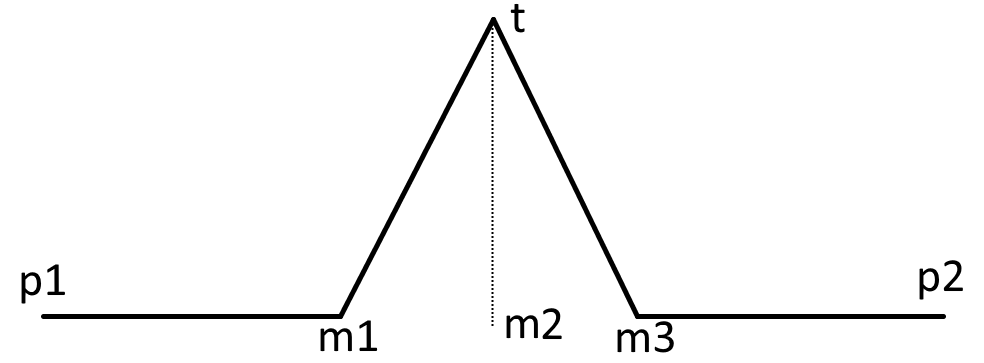
\includegraphics[width=\textwidth]{koch.png}
	\caption{Koch's curve gen 0}
	\label{fig:koch}
\end{figure}
Hierbij ligt \texttt{m2} midden tussen \texttt{p1} en \texttt{p2}.\\
De afstand tussen \texttt{p1} en \texttt{m1} is even groot als de afstand tussen \texttt{m2} en \texttt{t}.\\
\texttt{m1} ligt op $\frac{1}{3}$ afstand van \texttt{p1} naar \texttt{p2}.\\
\texttt{m3} ligt op $\frac{2}{3}$ afstand van \texttt{p1} naar \texttt{p2}.\\
\tip{Dit is een redelijk complexe opdracht. Teken dit eerst uit, en probeer al voordat je begint met coderen te weten \textit{wat} je precies gaat coderen. Maak gebruik van de \texttt{dist} \texttt{rotate} en \texttt{mult} PVector methods.}

\newpage
\section{[Bonus] Hilbert's Curve}
Maak de volgende functie:
\begin{lstlisting}
	void hilbertCurve(PVector p1,PVector p2) {
	} 
\end{lstlisting}
Die de volgende figuur (figuur \ref{fig:koch}) tekent:
\begin{figure}[H]
	\centering
	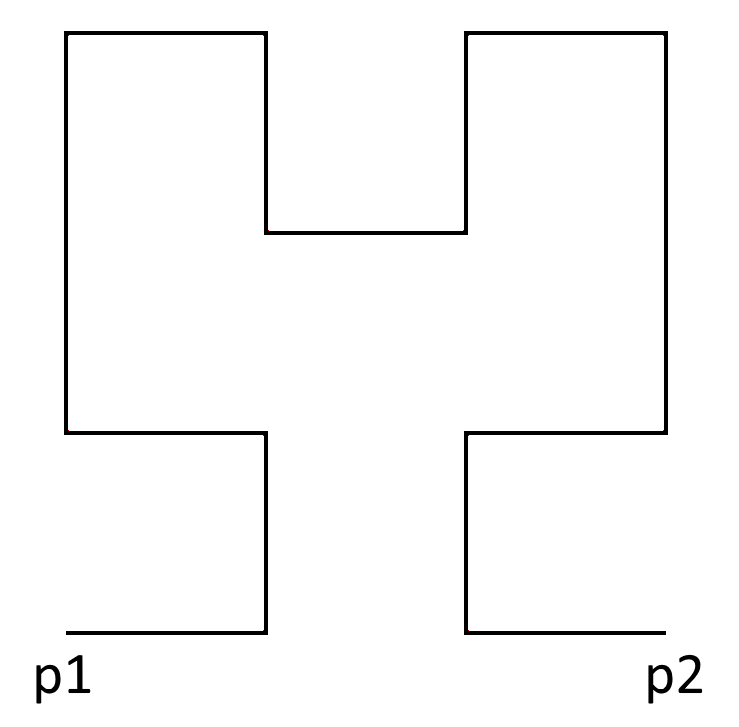
\includegraphics[width=4cm]{hilbert.png}
	\caption{Hilbert's Curve}
	\label{fig:koch}
\end{figure}

\end{document}